% Template for the submission to:
%   The Annals of Applied Statistics    [AOAS]
%
%%%%%%%%%%%%%%%%%%%%%%%%%%%%%%%%%%%%%%%%%%%%%%
%% In this template, the places where you   %%
%% need to fill in your information are     %%
%% indicated by '???'.                      %%
%%                                          %%
%% Please do not use \input{...} to include %%
%% other tex files. Submit your LaTeX       %%
%% manuscript as one .tex document.         %%
%%%%%%%%%%%%%%%%%%%%%%%%%%%%%%%%%%%%%%%%%%%%%%

\documentclass[aoas,preprint]{imsart}

%% Packages
\RequirePackage{amsthm,amsmath,amsfonts,amssymb}
\RequirePackage[authoryear]{natbib}
\usepackage{graphicx}
\usepackage{bm}
\usepackage{siunitx}
\usepackage{booktabs}
\usepackage{xcolor}
\usepackage{float}
\usepackage{commath}
\usepackage{fancybox}
\usepackage{tikz}
\usepackage{hyperref}
\usepackage{url}

% To work with loops and counters:
\usepackage{forloop}
\usepackage{calc}
\maxdeadcycles=10000

%\RequirePackage[colorlinks,citecolor=blue,urlcolor=blue]{hyperref}
%\RequirePackage{graphicx}% uncomment this for including figures

\startlocaldefs
%%%%%%%%%%%%%%%%%%%%%%%%%%%%%%%%%%%%%%%%%%%%%%
%%                                          %%
%% Uncomment next line to change            %%
%% the type of equation numbering           %%
%%                                          %%
%%%%%%%%%%%%%%%%%%%%%%%%%%%%%%%%%%%%%%%%%%%%%%
%\numberwithin{equation}{section}
%%%%%%%%%%%%%%%%%%%%%%%%%%%%%%%%%%%%%%%%%%%%%%
%%                                          %%
%% For Axiom, Claim, Corollary, Hypothezis, %%
%% Lemma, Theorem, Proposition              %%
%% use \theoremstyle{plain}                 %%
%%                                          %%
%%%%%%%%%%%%%%%%%%%%%%%%%%%%%%%%%%%%%%%%%%%%%%
%\theoremstyle{plain}
%\newtheorem{???}{???}
%\newtheorem*{???}{???}
%\newtheorem{???}{???}[???]
%\newtheorem{???}[???]{???}
%%%%%%%%%%%%%%%%%%%%%%%%%%%%%%%%%%%%%%%%%%%%%%
%%                                          %%
%% For Assumption, Definition, Example,     %%
%% Notation, Property, Remark, Fact         %%
%% use \theoremstyle{remark}                %%
%%                                          %%
%%%%%%%%%%%%%%%%%%%%%%%%%%%%%%%%%%%%%%%%%%%%%%
%\theoremstyle{remark}
%\newtheorem{???}{???}
%\newtheorem*{???}{???}
%\newtheorem{???}{???}[???]
%\newtheorem{???}[???]{???}
%%%%%%%%%%%%%%%%%%%%%%%%%%%%%%%%%%%%%%%%%%%%%%
%% Please put your definitions here:        %%
%%%%%%%%%%%%%%%%%%%%%%%%%%%%%%%%%%%%%%%%%%%%%%

\newcommand{\mysize}{0.4}

\endlocaldefs

\begin{document}

\begin{frontmatter}
%%%%%%%%%%%%%%%%%%%%%%%%%%%%%%%%%%%%%%%%%%%%%%
%%                                          %%
%% Enter the title of your article here     %%
%%                                          %%
%%%%%%%%%%%%%%%%%%%%%%%%%%%%%%%%%%%%%%%%%%%%%%
\title{Supplementary Material (3/3): SIMULATIONS}
%\title{A sample article title with some additional note\thanksref{T1}}
\runtitle{Supplementary Material}
%\thankstext{T1}{A sample of additional note to the title.}

\begin{aug}
%%%%%%%%%%%%%%%%%%%%%%%%%%%%%%%%%%%%%%%%%%%%%%
%%Only one address is permitted per author. %%
%%Only division, organization and e-mail is %%
%%included in the address.                  %%
%%Additional information can be included in %%
%%the Acknowledgments section if necessary. %%
%%%%%%%%%%%%%%%%%%%%%%%%%%%%%%%%%%%%%%%%%%%%%%
\author[A]{\fnms{Renzo} \snm{Caballero}\ead[label=e1]{Renzo.CaballeroRosas@kaust.edu.sa}},
\author[B]{\fnms{Ahmed} \snm{Kebaier}\ead[label=e2,mark]{kebaier@math.univ-paris13.fr}},
\author[C]{\fnms{Marco} \snm{Scavino}\ead[label=e3,mark]{mscavino@iesta.edu.uy}}
\and
\author[D]{\fnms{Ra\'ul} \snm{Tempone}\ead[label=e4,mark]{tempone@uq.rwth-aachen.de}}
%%%%%%%%%%%%%%%%%%%%%%%%%%%%%%%%%%%%%%%%%%%%%%
%% Addresses                                %%
%%%%%%%%%%%%%%%%%%%%%%%%%%%%%%%%%%%%%%%%%%%%%%
\address[A]{CEMSE Division, King Abdullah University of Science and Technology, Saudi Arabia, \printead{e1}}
\address[B]{Universit\'e Sorbonne Paris Nord, LAGA, CNRS, UMR 7539, F-93430, Villetaneuse, France, \printead{e2}}
\address[C]{Instituto de Estad\'{\i}stica (IESTA), Universidad de la Rep\'ublica, Montevideo, Uruguay, \printead{e3}}
\address[D]{Chair of Mathematics for Uncertainty Quantification, RWTH Aachen University, Germany, \printead{e4}}
\end{aug}

\begin{abstract}
In this material, we provide the simulation-based results corresponding to the forecast provider A. First, given the calibrated SDE Model 2 using a training dataset with 73 non-contiguous segments, each 24-hours long, we show simulated wind power production paths and empirical pointwise confidence bands for the wind power production in all the 74 non-contiguous segments of the testing dataset. Then, we show the results obtained by swapping the training dataset's roles and the testing dataset.
\end{abstract}

\begin{keyword}
\kwd{Wind Power}
\kwd{Probabilistic Forecasting}
\kwd{Stochastic Differential Equations}
\kwd{Lamperti Transform}
\kwd{Numerical Optimization}
\kwd{Model Selection}
\kwd{Time-Inhomogeneous Jacobi Diffusion}
\end{keyword}

\end{frontmatter}
%%%%%%%%%%%%%%%%%%%%%%%%%%%%%%%%%%%%%%%%%%%%%%
%% Please use \tableofcontents for articles %%
%% with 50 pages and more                   %%
%%%%%%%%%%%%%%%%%%%%%%%%%%%%%%%%%%%%%%%%%%%%%%
%\tableofcontents

%%%%%%%%%%%%%%%%%%%%%%%%%%%%%%%%%%%%%%%%%%%%%%
%%%% Main text entry area:

\tableofcontents

\newpage

\section{Provider A - Paths Simulations over testing forecast}
\quad
\graphicspath{{./plots/forecast_from_testing/paths/}}

\newcounter{i}
\newcounter{j}

\forloop{i}{0}{\value{i} < 9}{

\begin{figure}[!htb]
\centering
\setcounter{j}{\value{i}*8+1}
{\includegraphics[width=\mysize\columnwidth]{\arabic{j}.eps}}\quad
\setcounter{j}{\value{i}*8+2}
{\includegraphics[width=\mysize\columnwidth]{\arabic{j}.eps}}\\
\quad\\
\setcounter{j}{\value{i}*8+3}
{\includegraphics[width=\mysize\columnwidth]{\arabic{j}.eps}}\quad
\setcounter{j}{\value{i}*8+4}
{\includegraphics[width=\mysize\columnwidth]{\arabic{j}.eps}}\\
\quad\\
\setcounter{j}{\value{i}*8+5}
{\includegraphics[width=\mysize\columnwidth]{\arabic{j}.eps}}\quad
\setcounter{j}{\value{i}*8+6}
{\includegraphics[width=\mysize\columnwidth]{\arabic{j}.eps}}\\
\quad\\
\setcounter{j}{\value{i}*8+7}
{\includegraphics[width=\mysize\columnwidth]{\arabic{j}.eps}}\quad
\setcounter{j}{\value{i}*8+8}
{\includegraphics[width=\mysize\columnwidth]{\arabic{j}.eps}}
\end{figure}

\newpage

}

\begin{figure}[!htb]
\centering
{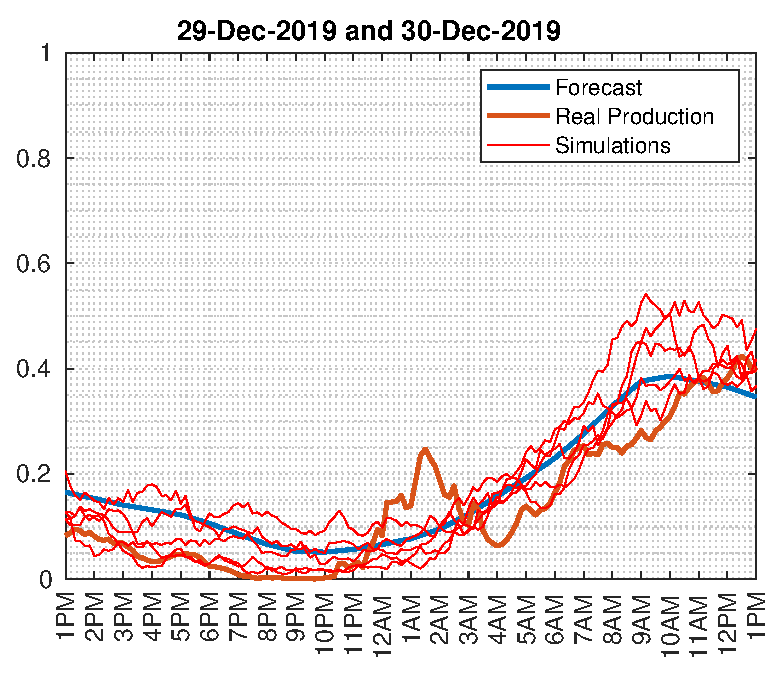
\includegraphics[width=\mysize\columnwidth]{73.eps}}\quad
{\includegraphics[width=\mysize\columnwidth]{74.eps}}\\
\end{figure}

\newpage

\section{Provider A - Probabilistic Bands Simulations over testing forecast}
\quad
\graphicspath{{./plots/forecast_from_testing/bands/}}

\forloop{i}{0}{\value{i} < 9}{

\begin{figure}[!htb]
\centering
\setcounter{j}{\value{i}*8+1}
{\includegraphics[width=\mysize\columnwidth]{\arabic{j}.eps}}\quad
\setcounter{j}{\value{i}*8+2}
{\includegraphics[width=\mysize\columnwidth]{\arabic{j}.eps}}\\
\quad\\
\setcounter{j}{\value{i}*8+3}
{\includegraphics[width=\mysize\columnwidth]{\arabic{j}.eps}}\quad
\setcounter{j}{\value{i}*8+4}
{\includegraphics[width=\mysize\columnwidth]{\arabic{j}.eps}}\\
\quad\\
\setcounter{j}{\value{i}*8+5}
{\includegraphics[width=\mysize\columnwidth]{\arabic{j}.eps}}\quad
\setcounter{j}{\value{i}*8+6}
{\includegraphics[width=\mysize\columnwidth]{\arabic{j}.eps}}\\
\quad\\
\setcounter{j}{\value{i}*8+7}
{\includegraphics[width=\mysize\columnwidth]{\arabic{j}.eps}}\quad
\setcounter{j}{\value{i}*8+8}
{\includegraphics[width=\mysize\columnwidth]{\arabic{j}.eps}}
\end{figure}

\newpage

}

\begin{figure}[!htb]
\centering
{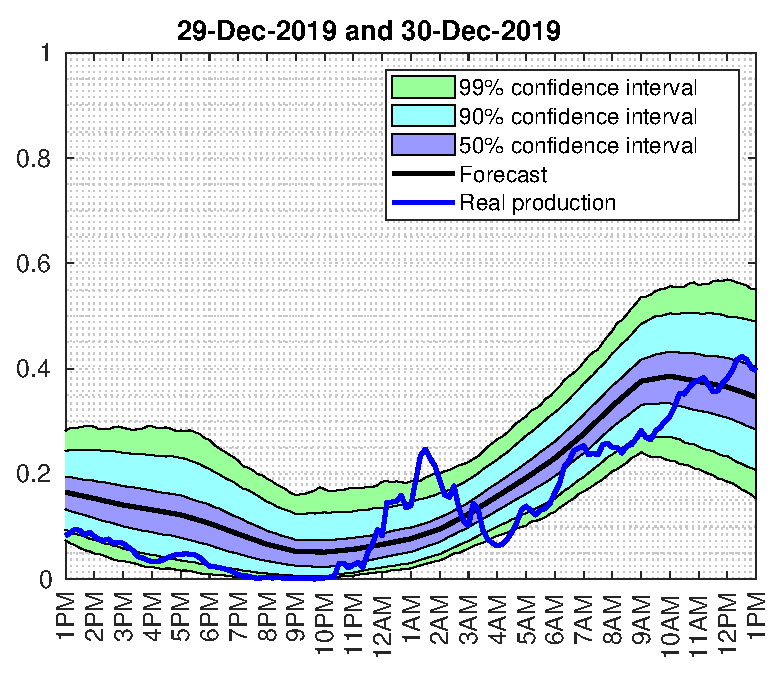
\includegraphics[width=\mysize\columnwidth]{73.eps}}\quad
{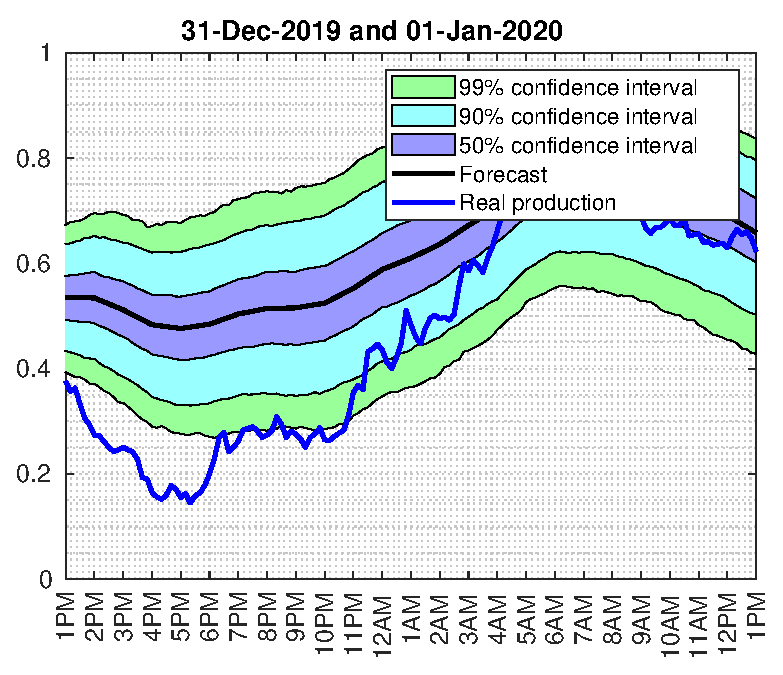
\includegraphics[width=\mysize\columnwidth]{74.eps}}\\
\end{figure}

\newpage

\section{Provider A - Paths Simulations over training forecast}
\quad
\graphicspath{{./plots/forecast_from_training/paths/}}

\forloop{i}{0}{\value{i} < 9}{

\begin{figure}[!htb]
\centering
\setcounter{j}{\value{i}*8+1}
{\includegraphics[width=\mysize\columnwidth]{\arabic{j}.eps}}\quad
\setcounter{j}{\value{i}*8+2}
{\includegraphics[width=\mysize\columnwidth]{\arabic{j}.eps}}\\
\quad\\
\setcounter{j}{\value{i}*8+3}
{\includegraphics[width=\mysize\columnwidth]{\arabic{j}.eps}}\quad
\setcounter{j}{\value{i}*8+4}
{\includegraphics[width=\mysize\columnwidth]{\arabic{j}.eps}}\\
\quad\\
\setcounter{j}{\value{i}*8+5}
{\includegraphics[width=\mysize\columnwidth]{\arabic{j}.eps}}\quad
\setcounter{j}{\value{i}*8+6}
{\includegraphics[width=\mysize\columnwidth]{\arabic{j}.eps}}\\
\quad\\
\setcounter{j}{\value{i}*8+7}
{\includegraphics[width=\mysize\columnwidth]{\arabic{j}.eps}}\quad
\setcounter{j}{\value{i}*8+8}
{\includegraphics[width=\mysize\columnwidth]{\arabic{j}.eps}}
\end{figure}

\newpage

}

\begin{figure}[!htb]
\centering
{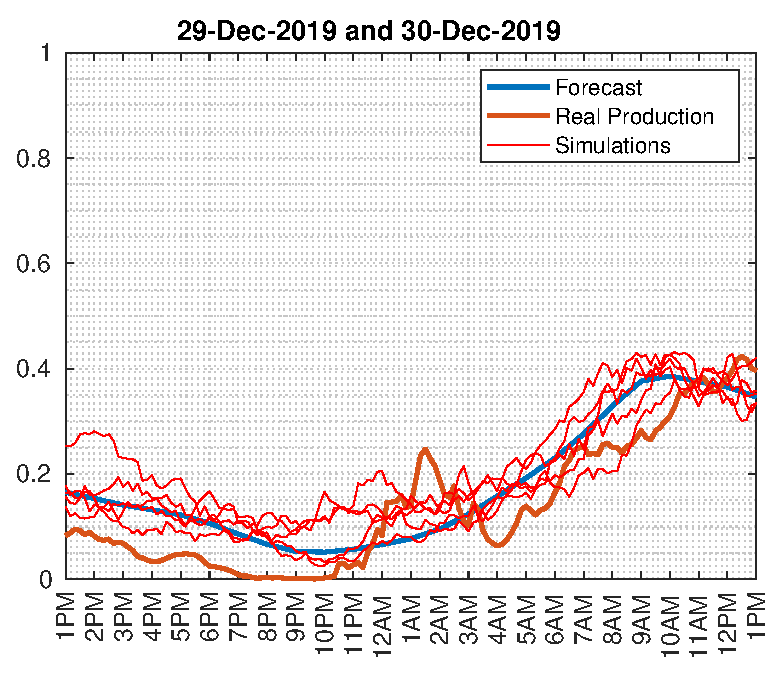
\includegraphics[width=\mysize\columnwidth]{73.eps}}
\end{figure}

\newpage

\section{Provider A - Probabilistic Bands Simulations over training forecast}
\quad
\graphicspath{{./plots/forecast_from_training/bands/}}

\forloop{i}{0}{\value{i} < 9}{

\begin{figure}[!htb]
\centering
\setcounter{j}{\value{i}*8+1}
{\includegraphics[width=\mysize\columnwidth]{\arabic{j}.eps}}\quad
\setcounter{j}{\value{i}*8+2}
{\includegraphics[width=\mysize\columnwidth]{\arabic{j}.eps}}\\
\quad\\
\setcounter{j}{\value{i}*8+3}
{\includegraphics[width=\mysize\columnwidth]{\arabic{j}.eps}}\quad
\setcounter{j}{\value{i}*8+4}
{\includegraphics[width=\mysize\columnwidth]{\arabic{j}.eps}}\\
\quad\\
\setcounter{j}{\value{i}*8+5}
{\includegraphics[width=\mysize\columnwidth]{\arabic{j}.eps}}\quad
\setcounter{j}{\value{i}*8+6}
{\includegraphics[width=\mysize\columnwidth]{\arabic{j}.eps}}\\
\quad\\
\setcounter{j}{\value{i}*8+7}
{\includegraphics[width=\mysize\columnwidth]{\arabic{j}.eps}}\quad
\setcounter{j}{\value{i}*8+8}
{\includegraphics[width=\mysize\columnwidth]{\arabic{j}.eps}}
\end{figure}

\newpage

}

\begin{figure}[!htb]
\centering
{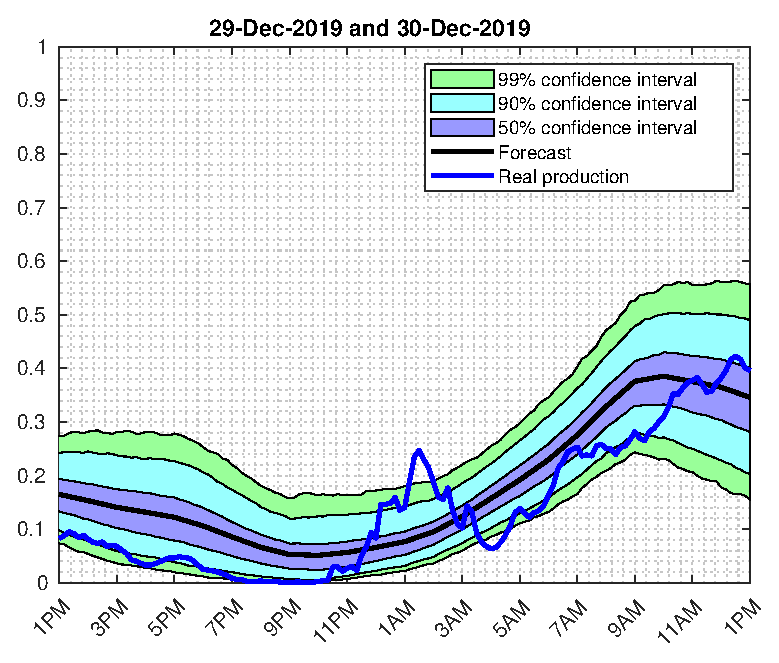
\includegraphics[width=\mysize\columnwidth]{73.eps}}
\end{figure}

\newpage

%%%%%%%%%%%%%%%%%%%%%%%%%%%%%%%%%%%%%%%%%%%%%%
%% Single Appendix:                         %%
%%%%%%%%%%%%%%%%%%%%%%%%%%%%%%%%%%%%%%%%%%%%%%
%\begin{appendix}
%\section*{???}%% if no title is needed, leave empty \section*{}.
%\end{appendix}
%%%%%%%%%%%%%%%%%%%%%%%%%%%%%%%%%%%%%%%%%%%%%%
%% Multiple Appendixes:                     %%
%%%%%%%%%%%%%%%%%%%%%%%%%%%%%%%%%%%%%%%%%%%%%%
%\begin{appendix}
%\section{???}
%
%\section{???}
%
%\end{appendix}

%%%%%%%%%%%%%%%%%%%%%%%%%%%%%%%%%%%%%%%%%%%%%%
%% Support information (funding), if any,   %%
%% should be provided in the                %%
%% Acknowledgements section.                %%
%%%%%%%%%%%%%%%%%%%%%%%%%%%%%%%%%%%%%%%%%%%%%%
% \section*{Acknowledgements}
% The authors would like to thank ...
% 
% The first author was supported by ...
% 
% The second author was supported in part by ...
 
%%%%%%%%%%%%%%%%%%%%%%%%%%%%%%%%%%%%%%%%%%%%%%
%% Supplementary Material, if any, should   %%
%% be provided in {supplement} environment  %%
%% with title inside \textbf{} and short    %%
%% description below.                       %%
%%%%%%%%%%%%%%%%%%%%%%%%%%%%%%%%%%%%%%%%%%%%%%
%\begin{supplement}
%\textbf{???}.
%???.
%\end{supplement}

%%%%%%%%%%%%%%%%%%%%%%%%%%%%%%%%%%%%%%%%%%%%%%%%%%%%%%%%%%%%%
%%                  The Bibliography                       %%
%%                                                         %%
%%  imsart-nameyear.bst  will be used to                   %%
%%  create a .BBL file for submission.                     %%
%%                                                         %%
%%  Note that the displayed Bibliography will not          %%
%%  necessarily be rendered by Latex exactly as specified  %%
%%  in the online Instructions for Authors.                %%
%%                                                         %%
%%  MR numbers will be added by VTeX.                      %%
%%                                                         %%
%%  Use \cite{...} to cite references in text.             %%
%%                                                         %%
%%%%%%%%%%%%%%%%%%%%%%%%%%%%%%%%%%%%%%%%%%%%%%%%%%%%%%%%%%%%%

%% if your bibliography is in bibtex format, uncomment commands:
%\bibliographystyle{imsart-nameyear} % Style BST file
%\bibliography{bibliography}       % Bibliography file (usually '*.bib')

%% or include bibliography directly:
% \begin{thebibliography}{}
% \bibitem[\protect\citeauthoryear{???}{???}]{b1}
% \end{thebibliography}

\end{document}
